\documentclass[12pt,a4paper]{article}
\usepackage[utf8]{inputenc}
\usepackage{graphicx}
\usepackage{tikz}
\usetikzlibrary{fit}
\usepackage{lmodern}
\usepackage{sectsty}


\sectionfont{\color{cyan}}

\begin{document}
    \begin{titlepage}
        {\fontfamily{lmss}\selectfont
        	\centering
        	
\includegraphics[width=0.30\textwidth]{logo.png}\par\vspace{1cm}
        	{\LARGE Capstone Project Demo 1 \par}
        	\vspace{0.25cm}
        	{\huge\bfseries \color{cyan}Test Report\par}
        	\vspace{1cm}
        	{\Large\textit{by} Brute Force\par}
            \vspace{0.25cm}
            \begin{tikzpicture}
                \node [inner sep=0pt,,outer sep=0pt,clip,rounded corners=0.5cm] (pict) at (0,0) {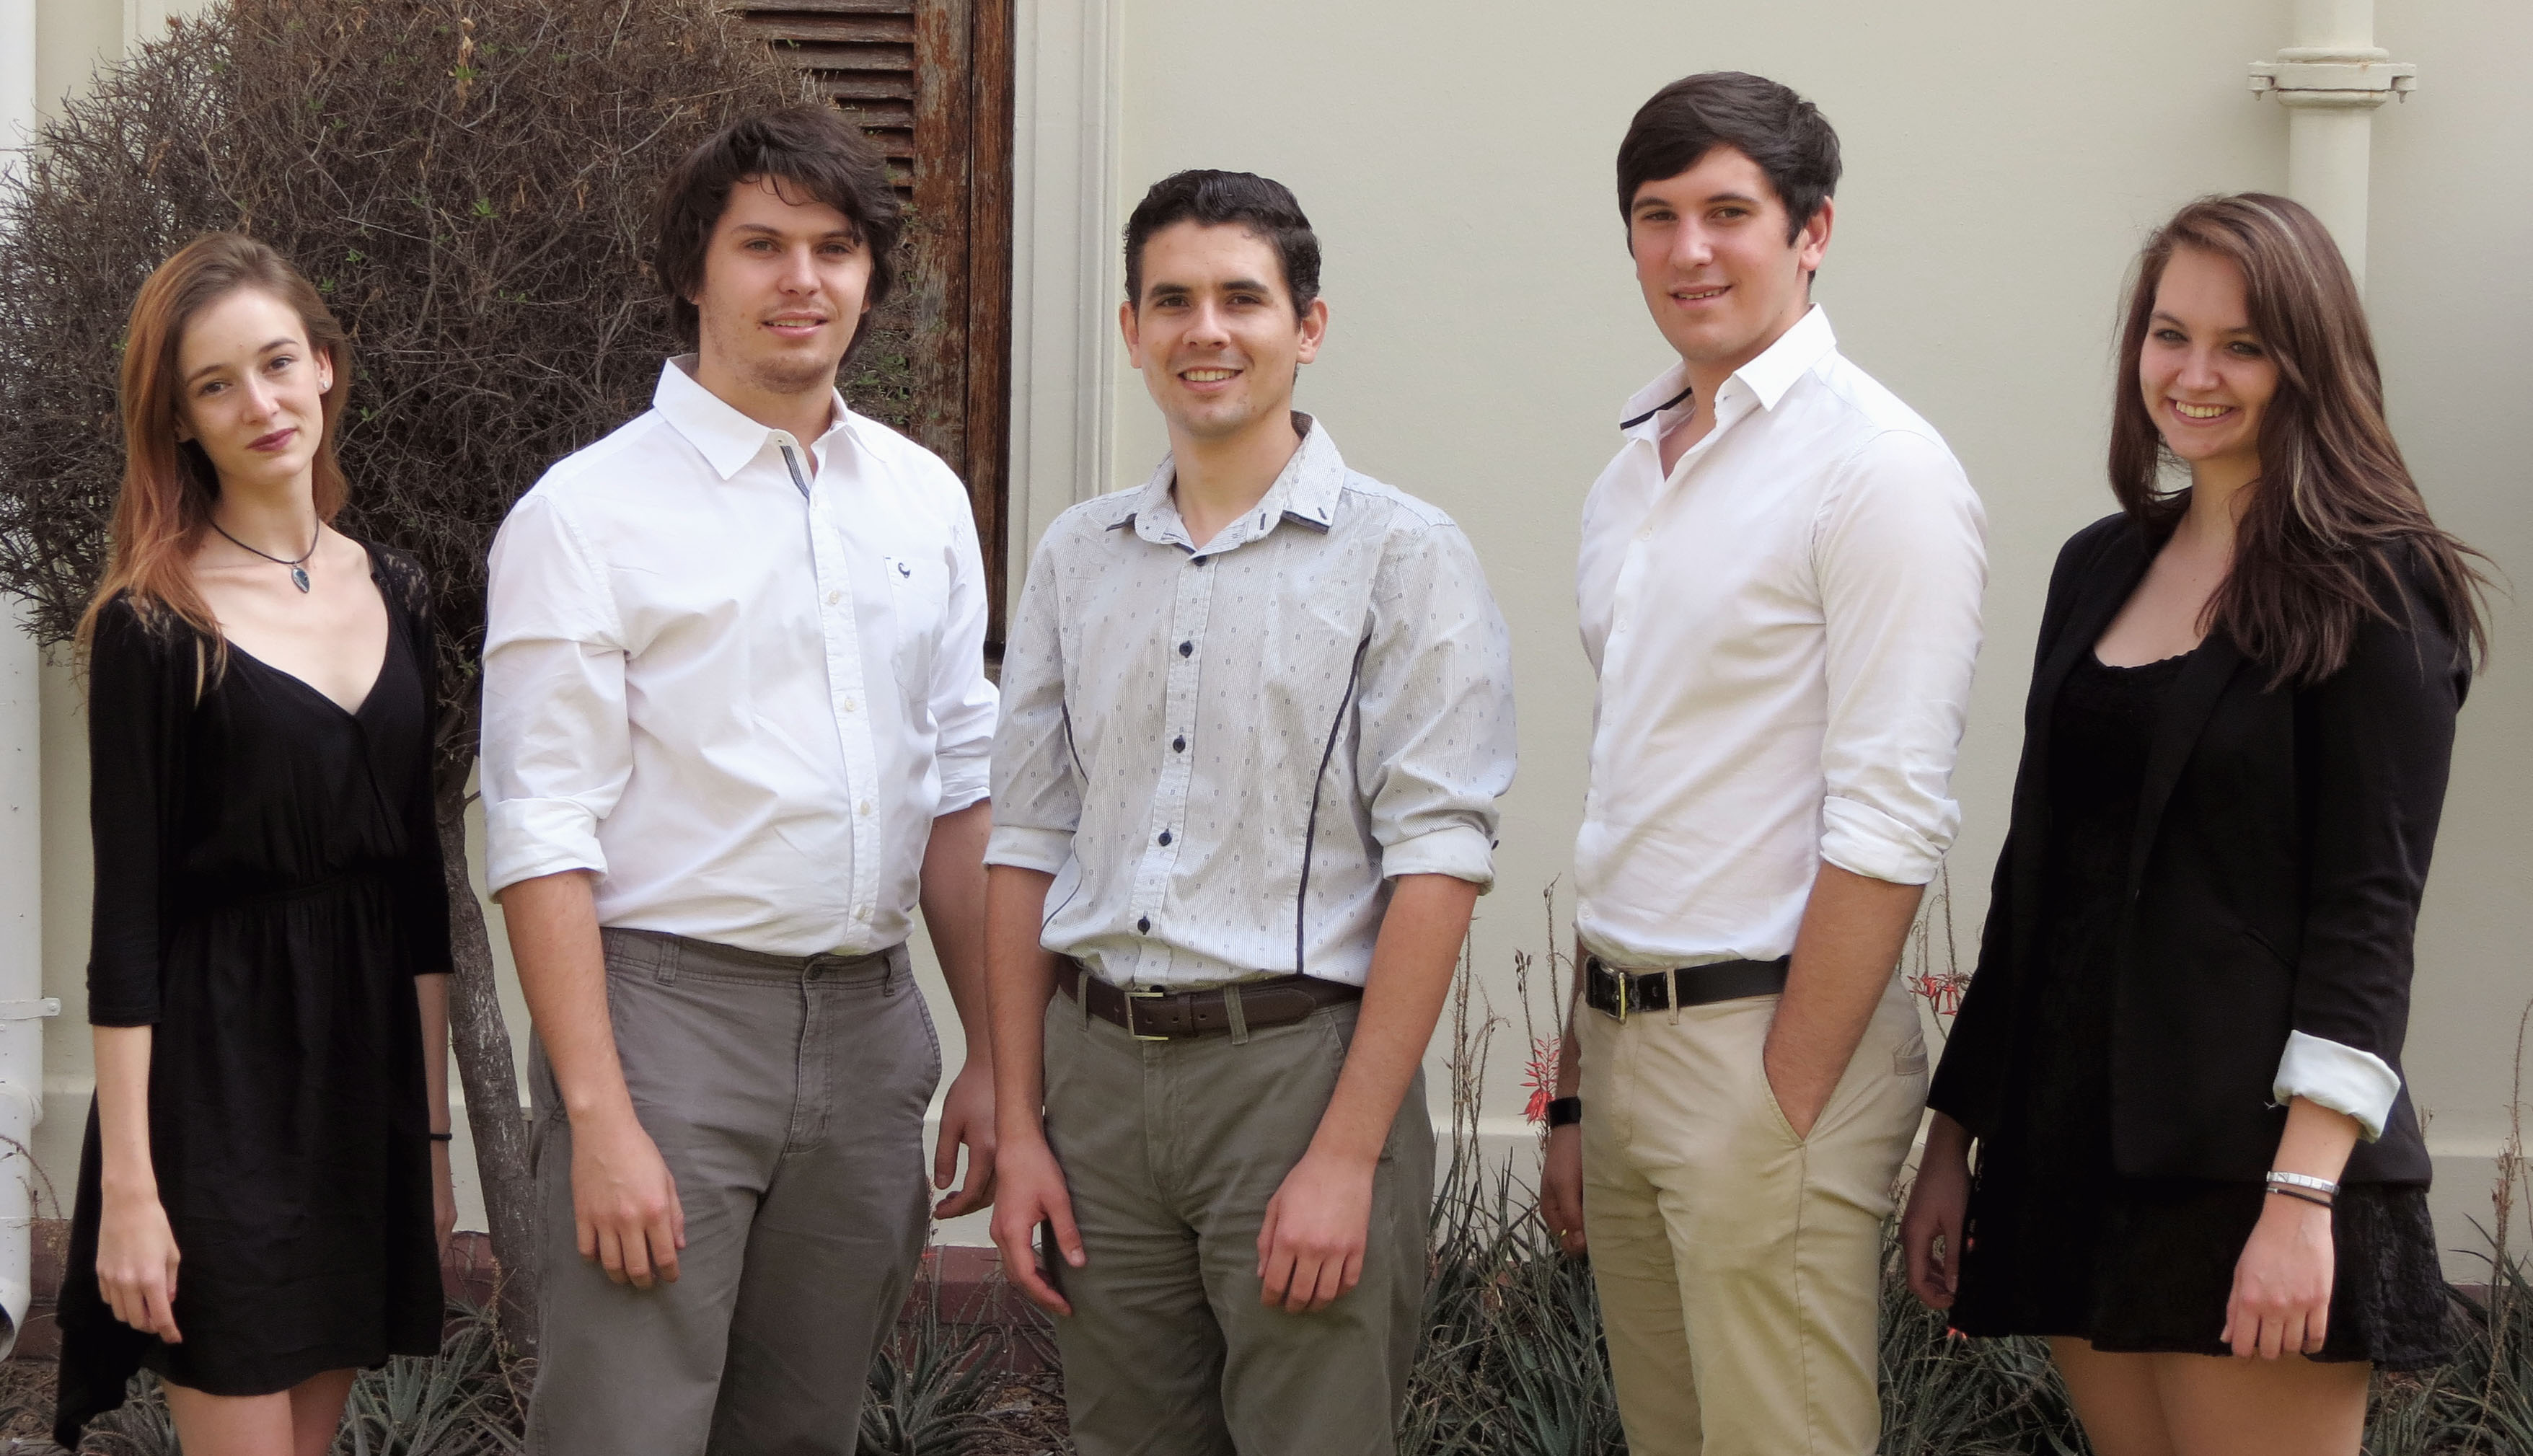
\includegraphics[width=0.9\textwidth]{team.jpg}};
                \node[fit=(pict),rounded corners=.55cm,inner sep=2pt]{};
            \end{tikzpicture}

            \par\vspace{1cm}
            \date{}
            \author{}
            \title{}
            \centering
            \textbf{Authors:}\\
            Mia Gerber\\
            Matthew Perry\\
            Wanrick Willemse\\
            Duart Breedt\\
            Linda Potgieter\\
        }
    \end{titlepage}
    \maketitle
    \tableofcontents
    \newpage

    \section{Introduction}
       	\subsection{Background}
            Here provide a summary of the aspects tested for this report.
        \subsection{Outline}
            Here provide a outline of this report.
        \subsection{Sources}
            Here provide a list of documents (if any) cited in this report.

    \section{Overview}
       	Here provide an overview of of the scope of the testing along with test environment detail (devices tested on and so forth.)
        Also specify the activities that are documented.

    \section{Variances}
        Here provide an overview of any deviances from the agreed upon testing process (Any aditional conditions tested and so forth.)

    \section{Evaluation}
        Here provide an overview of the comprehensiveness of the testing process (List all test cases that were run and list those that were not with an explanation.)

    \section{Results}
        Here provide an overview of the test results. List resolved issues with details and list outstanding issues.

\end{document}
